
\newglossaryentry{V-Modell 97}
{
    singular={V-Modell 97},
    plural={V-Modell 97},
    name={V-Modell 97},
    description={
        Eine Weiterentwicklung des \textbf{V-Modell nach Boehm} und empfohlenes Vorgehensmodell bei Softwareprojekten, die im Auftrag der BRD umgesetzt werden.\\
        Basiert auf 4 Submodellen: \textit{Projektmanagement}, \textit{Qualitätssicherung}, \textit{Systemerstellung}, \textit{Konfigurationsmanagement}\footnote{s. a. \url{https://t2informatik.de/wissen-kompakt/v-modell-97/}, abgerufen 26.03.2024)}
        2005 abgelöst durch \textbf{V-Modell XT}.
    }
}

\newglossaryentry{V-Modell nach Boehm}
{
    singular={V-Modell nach Boehm},
    plural={V-Modell nach Boehm},
    name={V-Modell nach Boehm},
    description={
        Vorgehensmodell bzw. Prozessreferenzmodell für die Softwareentwicklung (als \textit{Wasserfallmodell}), vorgeschlagen 1979 durch \textit{Barry Boehm}.
        \begin{figure}
            \centering
            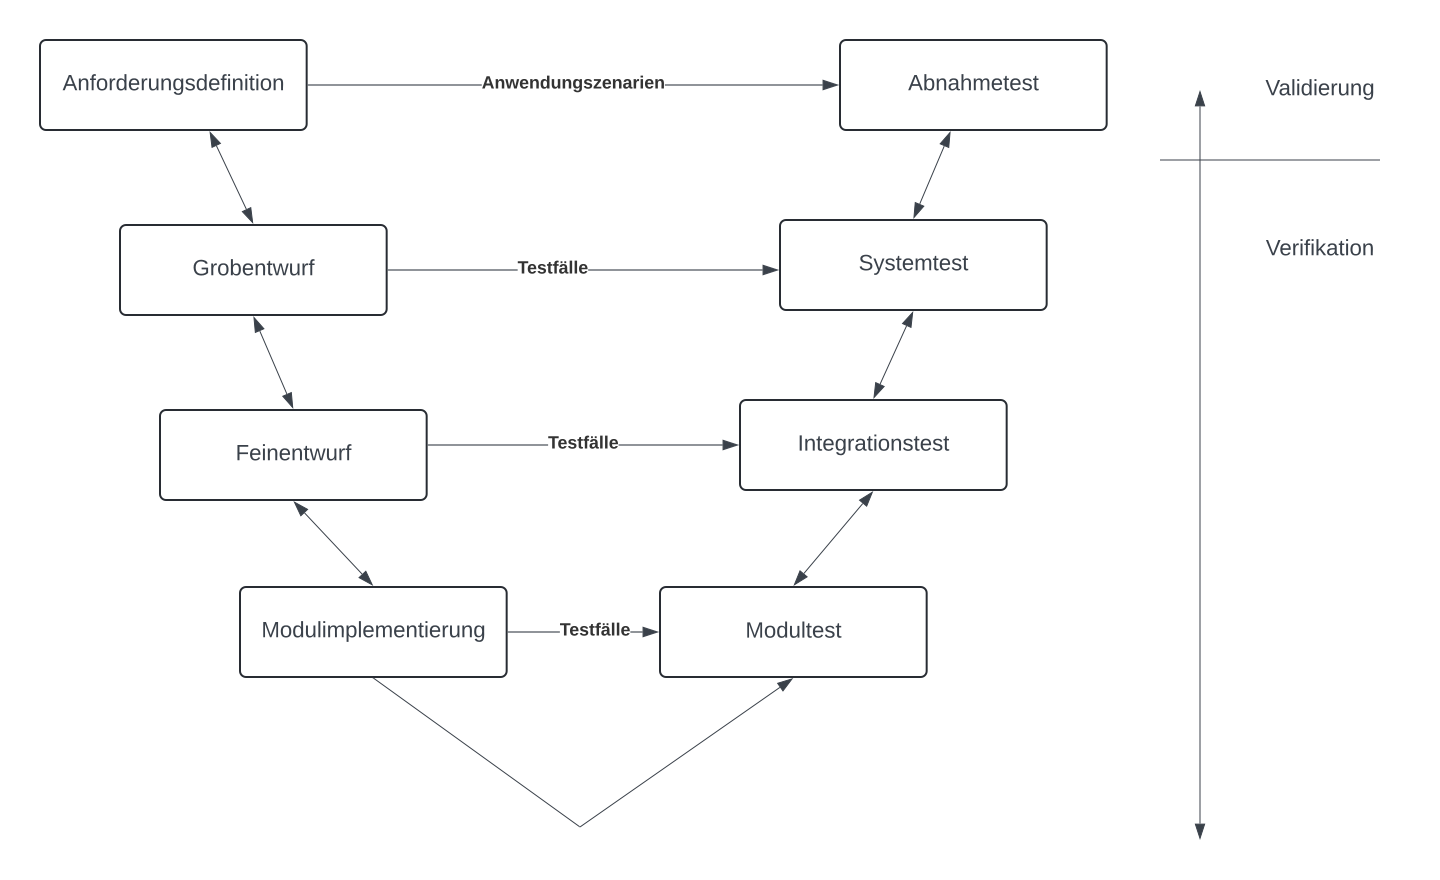
\includegraphics[scale=0.3]{chapters/Glossar/img/vmodell}
            \caption{Das Vorgehensmodell nach Boehm. (Quelle: in Anlehnung an \cite[329, Abbildung 14-7]{AABG14n})}
        \end{figure}
    }
}

\newglossaryentry{V-Modell XT}
{
    singular={V-Modell XT},
    plural={V-Modell XT},
    name={V-Modell XT},
    description={
        Weiterentwicklung des \textit{V-Modell 97}. Basiert auf aufeinander aufbauenden Vorgehensbausteinen, die die modularen EInheiten des V-Modells bilden. Verpflichtende Vorgehensbausteine als Kern des Modells betreffen das Projektmanagement, die Qualitätssicherung, das Konfigurstions-, Problem und Änderungsmanagement, die allesamt ein Mindestmaß von Projektdurchführungsqualität gewährleisten sollen. Das V-Modell XT ist mit 18 Vorgehensbausteinen weitaus feingranularer konzeptioniert, wodurch es leichter an Projektspezifika anzupassen ist (``\textit{Tailoring}``) als das V-Modell 97 (vgl.~\cite[329 f.]{AABG14n})
    }
}

\newglossaryentry{Tailoring}
{
    singular={Tailoring},
    plural={Tailoring},
    name={Tailoring},
    description={
        Projektspezifische Anpassung eines Phasenmodells an die konkrete Projektaufgabe  (vgl.~\cite[330]{AABG14n})
    }
}

\newglossaryentry{Team Software Process (TSP)}
{
    singular={Team Software Process (TSP)},
    plural={Team Software Process (TSP)},
    name={Team Software Process (TSP)},
    description={
        Der Team Software Prozess (TSP) ist eine Methode für Softwareentwicklungsteams zur Selbstoptimierung.
        [...]
        Durch die Verwendung von TSP sollen folgende Ziele erreicht werden:
        \begin{itemize}
            \item Bessere und genauere Planung (dadurch bessere Erfüllung von geplanten Daten)
            \item Verbesserung der Qualität des Produktes
            \item Niedrigere Kosten von Projekten (Total Cost of Ownership)}\footnote{
Quelle: \url{https://de.wikipedia.org/wiki/Team_Software_Process}, abgerufen 26.03.2024
}
        \end{itemize}
    }
}

\newglossaryentry{DV-Konzept}
{
singular={DV-Konzept},
plural={DV-Konzept},
name={DV-Konzept},
description={
\textit{Datenverarbeitungskonzept}. Relevante Daten werden von dem Fachkonzept in ein Modell (Persistierung / Verarbeitung) für eine konkrete Datenbank und/ oder Programmiersprache überführt. Im Wasserfallmodell ist das die Fortführung des \textit{Fachkonzeptes} (aus der 2. Phase ``\textit{Analyse}``) in der dritten Phase ``\textit{Entwurf}``.
}
}
